\documentclass[11pt]{article}

\usepackage[margin=1in]{geometry}
\usepackage[T1]{fontenc}
\usepackage{lmodern}
\usepackage{microtype}
\usepackage{amsmath,amssymb,amsthm,mathtools}
\usepackage[dvipsnames]{xcolor}
\usepackage{tikz}
\usepackage{enumitem}
\usepackage[hidelinks]{hyperref}

\definecolor{courseblue}{HTML}{1F4E79}
\definecolor{lightblue}{HTML}{EAF2F8}
\definecolor{darkgray}{HTML}{333333}

\setlength{\parindent}{0pt}
\setlength{\parskip}{0.65em}
\setlist[itemize]{topsep=0.25em,itemsep=0.15em}

\theoremstyle{definition}
\newtheorem{definition}{Definition}
\newtheorem{example}{Example}
\theoremstyle{remark}
\newtheorem*{remark}{Remark}

\newcommand{\C}{\mathbb{C}}
\newcommand{\R}{\mathbb{R}}
\newcommand{\RePart}{\operatorname{Re}}
\newcommand{\ImPart}{\operatorname{Im}}

\begin{document}

\begin{center}
  \colorbox{lightblue}{%
    \begin{minipage}{0.94\textwidth}
      \vspace{0.55em}
      \begin{tabular*}{\textwidth}{@{\extracolsep{\fill}}lr}
        {\color{courseblue}\bfseries\LARGE Lecture 1} &
        {\color{courseblue}\bfseries\LARGE MATH 411}\\[0.35em]
        \textbf{Fall 2026} & \textbf{Date: Sep 2, 2026}\\
        & \textbf{Instructor: Manish Patnaik}
      \end{tabular*}
      \vspace{0.45em}
    \end{minipage}}
\end{center}

\section{Complex Numbers}

\begin{definition}
The set of \emph{complex numbers} is
\[
  \C=\{a+ib : a,b\in\R\},
\]
where $i^2=-1$.  For $z=a+ib$, we write
\[
  \RePart(z)=a \qquad\text{and}\qquad \ImPart(z)=b.
\]
\end{definition}

The set $\C$ comes with the following algebraic operations.  If
$z_1=a_1+ib_1$, $z_2=a_2+ib_2$, and $c\in\R$, then
\begin{align*}
  z_1+z_2
    &= (a_1+a_2)+i(b_1+b_2),\\
  c z_1
    &= ca_1+i(cb_1),\\
  z_1z_2
    &= (a_1+ib_1)(a_2+ib_2)\\
    &= (a_1a_2-b_1b_2)+i(b_1a_2+a_1b_2).
\end{align*}
The last identity follows by expanding and using $i^2=-1$.

The additive identity is $0$, and the multiplicative identity is $1$:
\[
  0+z=z+0=z,
  \qquad
  1\cdot z=z\cdot 1=z.
\]
We regard $\R$ as a subset of $\C$ by identifying $a\in\R$ with
$a+i0\in\C$.

\subsection{Complex Conjugation and Inverses}

\begin{definition}
If $z=a+ib$, its \emph{complex conjugate} is
\[
  \overline{z}=a-ib.
\]
\end{definition}

Multiplying a complex number by its conjugate gives
\[
  z\overline{z}=(a+ib)(a-ib)=a^2+b^2\in\R_{\ge 0}.
\]
If $z\ne 0$, then $z\overline z=a^2+b^2>0$, and hence
\[
  z^{-1}=\frac{\overline z}{a^2+b^2}.
\]
Thus every nonzero complex number has a multiplicative inverse.  In
particular, $\C$ is a field, much like $\R$.

\subsection{The Complex Plane and the Modulus}

We identify $\C$ with $\R^2$ by sending $z=a+ib$ to the point $(a,b)$.
Under this identification, the real part is the horizontal coordinate and
the imaginary part is the vertical coordinate.

\begin{center}
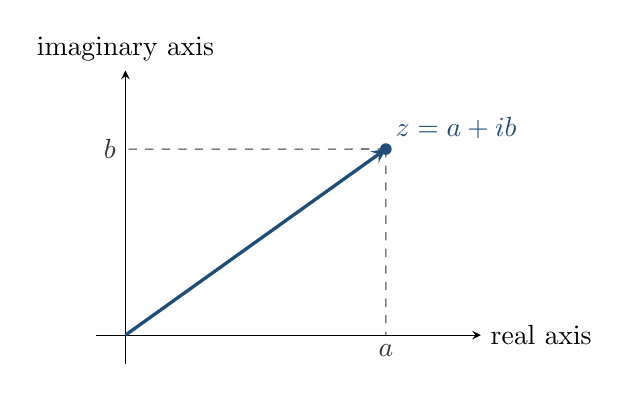
\begin{tikzpicture}[scale=1.05,>=stealth]
  \draw[->] (-0.35,0) -- (4.3,0) node[right] {real axis};
  \draw[->] (0,-0.35) -- (0,3.2) node[above] {imaginary axis};
  \coordinate (Z) at (3.15,2.25);
  \draw[very thick,courseblue,->] (0,0) -- (Z);
  \draw[dashed,darkgray] (Z) -- (3.15,0) node[below] {$a$};
  \draw[dashed,darkgray] (Z) -- (0,2.25) node[left] {$b$};
  \fill[courseblue] (Z) circle (2pt) node[above right] {$z=a+ib$};
\end{tikzpicture}
\end{center}

\begin{definition}
The \emph{modulus} (or absolute value) of $z=a+ib$ is
\[
  |z|=\sqrt{z\overline z}=\sqrt{a^2+b^2}.
\]
Geometrically, $|z|$ is the length of the vector in $\R^2$ represented by
$z$.
\end{definition}

The triangle inequality in $\R^2$ becomes the triangle inequality in $\C$:
\[
  |z_1+z_2|\le |z_1|+|z_2|.
\]
Addition of complex numbers is simply vector addition.

\begin{center}
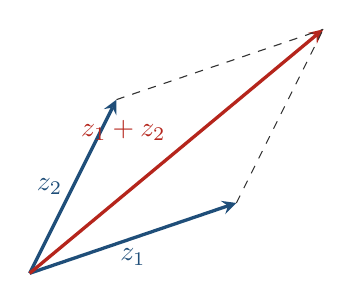
\begin{tikzpicture}[scale=1.05,>=stealth]
  \coordinate (O) at (0,0);
  \coordinate (A) at (2.5,0.85);
  \coordinate (B) at (1.05,2.1);
  \coordinate (S) at (3.55,2.95);
  \draw[->,very thick,courseblue] (O) -- (A) node[midway,below] {$z_1$};
  \draw[->,very thick,courseblue] (O) -- (B) node[midway,left] {$z_2$};
  \draw[->,very thick,BrickRed] (O) -- (S)
    node[midway,above left] {$z_1+z_2$};
  \draw[dashed,darkgray] (A) -- (S);
  \draw[dashed,darkgray] (B) -- (S);
\end{tikzpicture}
\end{center}

\section{Polar Form}

Let $z=a+ib\ne 0$.  Write $r=|z|$ and let $\theta$ be the angle measured
counterclockwise from the positive real axis to the vector representing $z$.
Then
\[
  a=r\cos\theta,
  \qquad
  b=r\sin\theta.
\]
Euler's formula is
\[
  e^{i\theta}=\cos\theta+i\sin\theta.
\]
It allows us to write $z$ in \emph{polar form}:
\[
  \boxed{z=re^{i\theta}}
  =r\cos\theta+i r\sin\theta.
\]
Here $r=|z|$ is the modulus of $z$, and $\theta$ is an argument of $z$.

\begin{center}
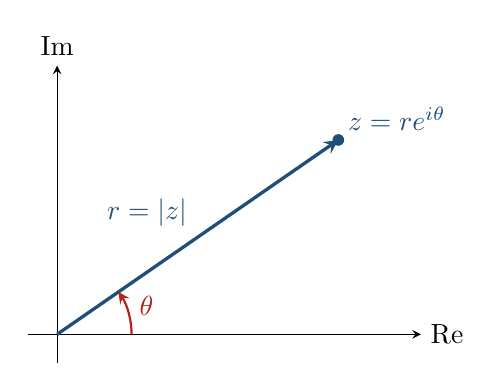
\begin{tikzpicture}[scale=1.05,>=stealth]
  \draw[->] (-0.35,0) -- (4.4,0) node[right] {$\RePart$};
  \draw[->] (0,-0.35) -- (0,3.25) node[above] {$\ImPart$};
  \coordinate (Z) at (3.4,2.35);
  \draw[very thick,courseblue,->] (0,0) -- (Z)
    node[midway,above left] {$r=|z|$};
  \fill[courseblue] (Z) circle (2pt) node[above right] {$z=re^{i\theta}$};
  \draw[BrickRed,thick,->] (0.9,0) arc[start angle=0,end angle=34.6,radius=0.9];
  \node[BrickRed] at (1.08,0.34) {$\theta$};
\end{tikzpicture}
\end{center}

Every $z\in\C\setminus\{0\}$ can be written as $z=re^{i\theta}$ with
$r>0$ and $\theta\in\R$.  The modulus $r$ is unique, while the argument is
unique only modulo $2\pi$:
\[
  e^{i(\theta+2\pi k)}=e^{i\theta}
  \qquad (k\in\mathbb Z).
\]
If we require $\theta\in[0,2\pi)$, then the argument is uniquely specified.

\subsection{Multiplication in Polar Form}

Suppose
\[
  z_1=re^{i\theta}
  \qquad\text{and}\qquad
  z_2=se^{i\varphi}.
\]
Then
\[
  z_1z_2=(rs)e^{i(\theta+\varphi)}.
\]
Thus multiplication of complex numbers \emph{multiplies moduli and adds
arguments}.

To verify this directly, expand using Euler's formula:
\begin{align*}
  e^{i\theta}e^{i\varphi}
  &= (\cos\theta+i\sin\theta)(\cos\varphi+i\sin\varphi)\\
  &= \bigl(\cos\theta\cos\varphi-\sin\theta\sin\varphi\bigr)\\
  &\qquad
     +i\bigl(\sin\theta\cos\varphi+\cos\theta\sin\varphi\bigr)\\
  &= \cos(\theta+\varphi)+i\sin(\theta+\varphi)\\
  &= e^{i(\theta+\varphi)}.
\end{align*}

\section{The Complex Exponential}

\begin{definition}
For $z=a+ib\in\C$, define
\[
  e^z=e^a e^{ib}.
\]
\end{definition}

The familiar exponential law continues to hold:
\[
  e^\alpha e^\beta=e^{\alpha+\beta}
  \qquad (\alpha,\beta\in\C).
\]

\begin{remark}
For complex $z$, the number $e^z$ need not be real or positive.  In fact,
$e^{ib}$ lies on the unit circle.
\end{remark}

\section{The \texorpdfstring{$n$}{n}-th Roots of a Complex Number}

\begin{example}
Let $z\in\C\setminus\{0\}$ and let $n$ be a positive integer.  We solve
\[
  w^n=z.
\]
Write
\[
  w=te^{i\varphi}
  \qquad\text{and}\qquad
  z=re^{i\theta},
\]
where $t,r>0$.  Then
\[
  w^n=t^n e^{in\varphi}=re^{i\theta}.
\]
Comparing moduli gives $t^n=r$, so $t=r^{1/n}$.  Comparing arguments modulo
$2\pi$ gives
\[
  n\varphi=\theta+2\pi k,
  \qquad\text{so}\qquad
  \varphi=\frac{\theta}{n}+\frac{2\pi k}{n}.
\]
Consequently, the $n$ distinct solutions are
\[
  \boxed{
    w_k=r^{1/n}
    e^{\,i\left(\frac{\theta}{n}+\frac{2\pi k}{n}\right)}
  },
  \qquad k=0,1,\ldots,n-1.
\]
\end{example}

The points $w_0,\ldots,w_{n-1}$ are equally spaced on the circle of radius
$r^{1/n}$, so they form the vertices of a regular $n$-gon.

\begin{center}
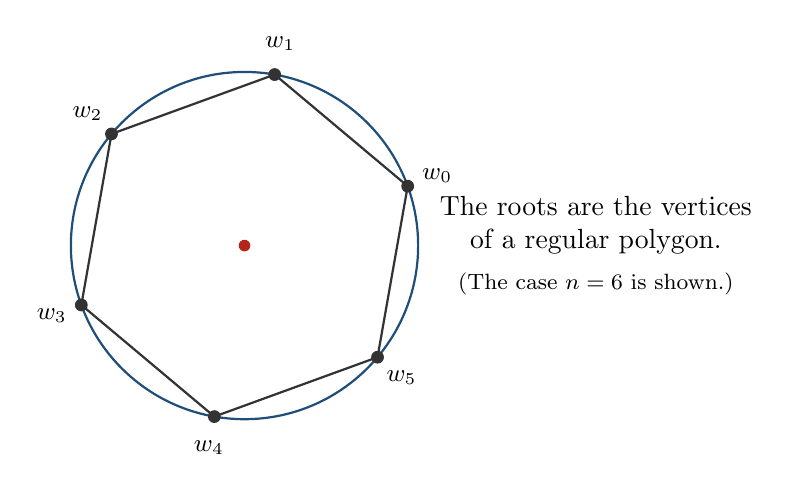
\begin{tikzpicture}[scale=1.05]
  \draw[courseblue,thick] (0,0) circle (2.1);
  \fill[BrickRed] (0,0) circle (2pt);
  \foreach \k in {0,...,5} {
    \coordinate (P\k) at ({20+60*\k}:2.1);
    \fill[darkgray] (P\k) circle (2.2pt);
    \node[font=\small] at ({20+60*\k}:2.48) {$w_{\k}$};
  }
  \draw[darkgray,thick]
    (P0) -- (P1) -- (P2) -- (P3) -- (P4) -- (P5) -- cycle;
  \node[align=center] at (4.25,0) {The roots are the vertices\\of a regular polygon.\\[0.3em]
    \footnotesize (The case $n=6$ is shown.)};
\end{tikzpicture}
\end{center}

\end{document}
